% Provenance (never printed): see sources/outline_sources.md (Year 2: energy geology --- the
% petroleum system quantified, unconventional resources, geothermal systems, uranium deposits,
% geological storage of carbon dioxide).
% Kerogen kinetics and elemental analyses: Fletcher and Pugmire (DOE, OSTI 1176871); kerogen
% types and Easy%Ro: Advanced Chemistry Basins Project (DOE, OSTI 830009); maturity thresholds:
% USGS MF-2008-B; TTI: Waples (1980) and Hammerschmidt et al. (2014); volumetrics and CO2
% storage: DOE/NETL (2008) and IPCC SRCCS (2005) chapter 5; geothermal: USGS OFR 2008-1296 and
% FS 2008-3082; uranium: USGS Bulletin 1693; Oklo: OSTI abstract records. Ledger rows in
% sources/ledger/book4.md; curves from figdata/bachelor-2/maturation.py and co2_density.py,
% numbers from the Book 4 second-writer scratch calculator calc/ch30.py.
% Geology and sourced numbers only: no advocacy, no policy.
\chapter{Geología de la energía}\label{ch:b2:energy-geology}

El petróleo es el resto de organismos microscópicos, enterrados con fango y cocidos durante millones de años a
unos \qty{100}{\celsius}; la energía geotérmica es ese mismo calor de la Tierra, aprovechado directamente.
Ambos están regidos por la temperatura y el tiempo: el primero, por la velocidad a la que avanza una reacción química a medida que
las rocas enterradas se calientan lentamente; la segunda, por cuánto calor almacena un volumen de roca y con qué rapidez el agua
puede llevarlo hasta un pozo. Este capítulo cuantifica el sistema petrolífero, pasa a los recursos a los que
les falta uno de sus elementos, al calor geotérmico y al uranio, y termina con la operación inversa:
devolver el dióxido de carbono al subsuelo.
% ledger: earle:oil-window, earle:organic-preservation

\begin{recall}
\textbf{De los volúmenes escolares}: roca generadora, querógeno, maduración, ventana del petróleo, migración,
roca almacén, roca sello, trampa, roca de sobrecarga, sistema petrolífero; carbón y rango del carbón; energía geotérmica.
\textbf{Del volumen de primer año}: flujo de calor y geoterma; porosidad y permeabilidad; presión del fluido
intersticial, esfuerzo efectivo y criterio de Coulomb; registro de sondeo; cuenca sedimentaria y
subsidencia. \textbf{De los libros de química}: la ley de Arrhenius, la energía de activación, la reacción de primer
orden. \textbf{De los libros de física}: la desintegración radiactiva, la constante de desintegración, el periodo de semidesintegración; el
punto crítico de un fluido. \textbf{Del \cref{ch:b2:basins-compared}}: \omterm{def:b2:basins-compared:curve}{curva de subsidencia}.
\textbf{Del \cref{ch:b2:ore-deposits}}: \omterm{def:b2:ore-deposits:types}{tipo de yacimiento}, \omterm{def:b2:ore-deposits:grade}{tonelaje}.
\end{recall}

\section{El sistema petrolífero cuantificado}\label{sec:b2:energy-geology:petroleum}

Un sistema petrolífero necesita una roca generadora rica en querógeno, una roca almacén, una roca sello, una trampa y una
sobrecarga suficiente para calentar la roca generadora, y sus sucesos deben producirse en el orden correcto: la trampa debe
existir cuando el petróleo migra. Cuantificarlo significa responder a tres preguntas: qué \omterm{def:b2:energy-geology:kerogen}{tipo de querógeno}
contiene la roca generadora, en qué medida se ha transformado y qué parte del producto se encuentra en la
trampa.
% ledger: magoon00:tps

\begin{definition}[Tipo de querógeno, diagrama de van Krevelen]\label{def:b2:energy-geology:kerogen}
Los querógenos se dividen en tres \emph{tipos de querógeno}\index{tipo de querogeno@tipo de querógeno} según su composición elemental:
el tipo~I, sapropélico, el más rico en hidrógeno, que genera sobre todo petróleo; el tipo~III, húmico o carbonoso,
pobre en hidrógeno, que genera sobre todo metano; y el tipo~II, intermedio, fuente tanto de petróleo
como de gas. El \emph{diagrama de van Krevelen}\index{diagrama de van Krevelen} representa la razón atómica H/C de
un querógeno frente a su razón atómica O/C; los tipos ocupan regiones distintas de él, y la maduración
desplaza un querógeno hacia valores bajos de H/C y de O/C.
\end{definition}

Siete querógenos inmaduros de tipo conocido, analizados en un mismo estudio de laboratorio, tienen razones atómicas H/C de
1.51 y 1.61 (tipo~I, entre ellos la lutita bituminosa de Green River, en Utah, depositada en lagos y rica en
restos de algas), de 1.22 a 1.28 (tipo~II, entre ellos la Kimmeridge Clay del mar del Norte),
1.13 (un tipo mixto~II/III) y 0.99 (tipo~III, el carbón de Cameo, en Colorado). El querógeno de Green
River, con un \qty{77}{\percent} de carbono en masa, tiene una composición media C$_{100}$H$_{150}$N$_3$O$_8$S: H/C 1.50 y
O/C 0.08. Calentado en el laboratorio a \qty{10}{K} por minuto, deja un residuo cuyo H/C baja a
1.20 a \qty{460}{\celsius} y a 0.54 a \qty{525}{\celsius}, mientras su O/C baja de 0.08 a alrededor de
0.01: la trayectoria dibujada a la izquierda de la figura siguiente.
% ledger: acb04:kerogens, fp14:gr-kerogen, fp14:gr-chars, mf88:thresholds
% values: GR3.9 kerogen H/C 1.486, O/C 0.080; chars 460 C 1.200/0.016, 525 C 0.544/0.011 (figdata maturation.py vk)

\begin{omfigure}
\centering
\begin{minipage}[b]{0.49\linewidth}\centering
\begin{tikzpicture}
\begin{axis}[omrecord, width=0.95\linewidth, height=5.0cm, xmin=0, xmax=0.12, ymin=0, ymax=1.8,
  xlabel={O/C atómico}, ylabel={H/C atómico}, xtick={0,0.04,0.08}, scaled x ticks=false,
  xticklabel style={/pgf/number format/fixed}, tick label style={font=\scriptsize},
  label style={font=\small}]
% computed in figdata/bachelor-2/maturation.py part vk; ledger: fp14:gr-kerogen, fp14:gr-chars
\addplot[omThm, line width=0.9pt, mark=*, mark size=1.3pt, -{Stealth[length=4pt]}] table[x=oc, y=hc] {figdata/out/bachelor-2-maturation-vk.dat};
\node[font=\scriptsize, text=omThm, anchor=north east] at (axis cs:0.081,1.45) {querógeno};
\node[font=\scriptsize, text=omThm, anchor=west] at (axis cs:0.013,0.52) {\qty{525}{\celsius}};
% ledger: acb04:kerogens (H/C of immature kerogens; O/C not reported)
\draw[omThm, line width=1pt] (axis cs:0.104,1.51) -- (axis cs:0.12,1.51);
\draw[omThm, line width=1pt] (axis cs:0.104,1.61) -- (axis cs:0.12,1.61);
\draw[omProp, line width=1pt] (axis cs:0.104,1.22) -- (axis cs:0.12,1.22);
\draw[omProp, line width=1pt] (axis cs:0.104,1.25) -- (axis cs:0.12,1.25);
\draw[omProp, line width=1pt] (axis cs:0.104,1.28) -- (axis cs:0.12,1.28);
\draw[omExo, line width=1pt] (axis cs:0.104,1.13) -- (axis cs:0.12,1.13);
\draw[omDef, line width=1pt] (axis cs:0.104,0.99) -- (axis cs:0.12,0.99);
\node[font=\scriptsize, text=omThm, anchor=east] at (axis cs:0.103,1.58) {I};
\node[font=\scriptsize, text=omProp, anchor=east] at (axis cs:0.103,1.25) {II};
\node[font=\scriptsize, text=omDef, anchor=east] at (axis cs:0.103,0.97) {III};
\end{axis}
\end{tikzpicture}
\end{minipage}\hfill
\begin{minipage}[b]{0.49\linewidth}\centering
\begin{tikzpicture}
\begin{axis}[omrecord, width=0.95\linewidth, height=5.0cm, xmin=60, xmax=220, ymin=0, ymax=1,
  xlabel={temperatura (\unit{\celsius})}, ylabel={tasa de transformación},
  tick label style={font=\scriptsize}, label style={font=\small}]
% computed in figdata/bachelor-2/maturation.py part tr; ledger: fp14:gr-daem
\addplot[black!40, densely dotted] coordinates {(60,0.5) (220,0.5)};
\addplot[omDef, line width=1.1pt] table[x=t_c, y=tr1] {figdata/out/bachelor-2-maturation-tr.dat};
\addplot[omThm, line width=1.1pt] table[x=t_c, y=tr10] {figdata/out/bachelor-2-maturation-tr.dat};
\addplot[omDef, line width=0.6pt, densely dashed] table[x=t_c, y=app1] {figdata/out/bachelor-2-maturation-tr.dat};
\addplot[omThm, line width=0.6pt, densely dashed] table[x=t_c, y=app10] {figdata/out/bachelor-2-maturation-tr.dat};
\node[font=\scriptsize, text=omDef, anchor=east] at (axis cs:125,0.80) {\qty{1}{\celsius\per\Myr}};
\node[font=\scriptsize, text=omThm, anchor=west] at (axis cs:160,0.30) {\qty{10}{\celsius\per\Myr}};
\end{axis}
\end{tikzpicture}
\end{minipage}
\par\smallskip{\small Izquierda: un \omterm{def:b2:energy-geology:kerogen}{diagrama de van Krevelen}. La trayectoria roja es el querógeno de tipo~I de Green River
y sus residuos tras calentarlo en el laboratorio a \qty{10}{K} por minuto hasta 400--\qty{525}{\celsius};
las marcas de la derecha indican el H/C de siete querógenos inmaduros de tipo~I (rojo), II (naranja),
II/III (gris) y III (azul), cuyo O/C no se publicó. Datos: Fletcher y Pugmire (2014);
Advanced Chemistry Basins Project (2004). Derecha: tasa de transformación del querógeno de Green River
calentado a velocidad constante desde \qty{10}{\celsius}, con su distribución de energías de activación
(continua) y solo con su energía media, según \eqref{eq:b2:energy-geology:maturation} (discontinua).}
\end{omfigure}

La transformación del querógeno en petróleo es un conjunto de reacciones de primer orden, cada una de las cuales obedece la
ley de Arrhenius. En una cuenca que se hunde, la temperatura de una roca generadora sube lenta y casi
uniformemente, lo que hace del resultado siguiente el núcleo de los modelos de maduración.

\begin{proposition}[Reacción de primer orden con velocidad de calentamiento constante]\label{prop:b2:energy-geology:maturation}
Sea una reacción de primer orden de constante de velocidad $k = A\,e^{-E/RT}$ que avanza en un material calentado a la
velocidad constante $\beta = \mathrm{d}T/\mathrm{d}t$ desde una temperatura $T_0$ a la que $k$ es despreciable.
La fracción que queda sin transformar a la temperatura $T$ es
\begin{equation}
x(T) = \exp\Bigl[-\frac{A}{\beta}\int_{T_0}^{T} e^{-E/RT'}\,\mathrm{d}T'\Bigr]
\approx \exp\Bigl[-\frac{A R T^2}{\beta E}\,e^{-E/RT}\Bigr] ,
\label{eq:b2:energy-geology:maturation}
\end{equation}
y la aproximación es válida cuando $E/RT \gg 1$; la tasa de transformación es $1 - x$.
\end{proposition}

\begin{proof}
Primer orden significa $\mathrm{d}x/\mathrm{d}t = -k x$. Con $\mathrm{d}t = \mathrm{d}T/\beta$,
$\mathrm{d}\ln x = -(A/\beta)\,e^{-E/RT}\,\mathrm{d}T$, e integrar desde $x = 1$ en $T_0$ da
la primera forma. Para la integral, $\frac{\mathrm{d}}{\mathrm{d}T}\bigl[\frac{RT^2}{E}e^{-E/RT}\bigr]
= \bigl(1 + \frac{2RT}{E}\bigr)e^{-E/RT}$, así que la integral es igual a $\frac{RT^2}{E}e^{-E/RT}$ salvo una
corrección relativa del orden de $2RT/E$; el límite inferior no contribuye, ya que $e^{-E/RT_0} \ll
e^{-E/RT}$.
\end{proof}

De ello se siguen dos consecuencias. La transformación se produce en un intervalo estrecho de temperatura, porque
$e^{-E/RT}$ cambia muy deprisa (\cref{exo:b2:energy-geology:11}). Y un calentamiento más lento transforma
a menor temperatura: haciendo $x = 1/2$, una velocidad de calentamiento diez veces mayor eleva la temperatura de
semitransformación en alrededor de $(RT^2/E)\ln 10$. La cinética del querógeno de Green River, ajustada a la
pirólisis de laboratorio, es $A = \qty{9.21e13}{s^{-1}}$ y $E/R = \qty{26800}{K}$ ($E =
\qty{223}{kJ/mol}$); con esta energía única, la semitransformación se produce a \qty{136.4}{\celsius} para
\qty{1}{\celsius\per\Myr} y a \qty{150.9}{\celsius} para \qty{10}{\celsius\per\Myr}, un desplazamiento de
\qty{14.5}{\celsius} frente a los $6.26 \times \ln 10 = \qty{14.4}{K}$ previstos. Calentado a
\qty{10}{K} por minuto, el mismo querógeno se transforma cerca de \qty{450}{\celsius}
(\cref{exo:b2:energy-geology:6}): el tiempo sustituye a la temperatura, y por eso la cinética se
mide por pirólisis a unos 250 a \qty{600}{\celsius}, y por eso extrapolarla a lo largo de doce
órdenes de magnitud en la velocidad de calentamiento deja incierta la profundidad prevista de la ventana del petróleo.
% ledger: fp14:gr-daem, acb04:kinetic-spread, codata:R
% values: Thalf 136.403 / 150.873 C; RT2/E 6.2587 K; lab 445.9 C (figdata maturation.py numbers, calc/ch30.py)

Un querógeno real contiene enlaces de muy distintas energías, de modo que su cinética es una distribución de energías de
activación, y cada fracción obedece la proposición; para el querógeno de Green River la distribución es
normal, con una desviación típica $\sigma/R = \qty{481}{K}$. La distribución reparte la
transformación, como muestra la derecha de la figura: a \qty{150}{\celsius}, el querógeno calentado a
\qty{1}{\celsius\per\Myr} está transformado en un \qty{93}{\percent}, y el calentado diez veces más deprisa, en un
\qty{48}{\percent}.
% ledger: fp14:gr-daem
% values: TR 0.927 / 0.484 at 150 C (figdata maturation.py numbers)

\begin{definition}[Reflectancia de la vitrinita, índice tiempo--temperatura]\label{def:b2:energy-geology:maturity}
La \emph{reflectancia de la vitrinita}\index{reflectancia de la vitrinita}, $R_o$, es el porcentaje de la luz
incidente que reflejan granos pulidos de vitrinita, un componente orgánico del carbón y del querógeno,
medido al microscopio; aumenta de forma irreversible con el calentamiento y registra la madurez térmica máxima que ha alcanzado una roca. El
\emph{índice tiempo--temperatura}\index{indice tiempo--temperatura@índice tiempo--temperatura} (TTI, por sus siglas en inglés) de Lopatin es la suma
$\sum_n \Delta t_n\,2^n$ sobre los intervalos de \qty{10}{\celsius} que ha atravesado una roca,
siendo $\Delta t_n$ el tiempo en millones de años pasado en el intervalo de número $n$, con $n = 0$
para 100 a \qty{110}{\celsius}, $n = 1$ para 110 a \qty{120}{\celsius}, $n = -1$ para 90 a
\qty{100}{\celsius}, y así sucesivamente.
\end{definition}

En la escala de reflectancia, la generación de petróleo a partir de querógenos de tipo~I y II empieza cerca de $R_o =
\qty{0.60}{\percent}$; por encima del 1.20 al \qty{1.30}{\percent} el petróleo es inestable y se descompone en
metano; el tipo~III empieza a producir metano cerca del \qty{0.73}{\percent}, y la generación de gas continúa hasta
alrededor del \qty{4.8}{\percent}. Los modelos calculan $R_o$ como un querógeno: el modelo Easy\%Ro
trata la vitrinita como veinte reacciones de primer orden en paralelo con $A = \qty{e13}{s^{-1}}$ y energías
de 34 a \qty{72}{kcal/mol} (de 142 a \qty{301}{kJ/mol}), y transforma su fracción convertida $F$,
como máximo 0.85, en $R_o = \exp(-1.6 + 3.7F)$, que va de 0.20 a \qty{4.7}{\percent}.
% ledger: mf88:thresholds, acb04:easyro, fp14:gr-chars

La reflectancia se calcula del mismo modo a lo largo de cada horizonte de una cuenca. En la cuenca inventada de la
figura siguiente, el sedimento se acumuló a \qty{100}{m} por millón de años de 100 a \qty{70}{\Ma},
y después a \qty{35}{m} por millón de años, bajo una superficie a \qty{10}{\celsius} y con un gradiente constante
de \qty{30}{\celsius\per\km}. Su horizonte más antiguo alcanzó $R_o = \qty{0.6}{\percent}$ hace
\qty{67.6}{\Ma}, a \qty{3080}{m} y \qty{102}{\celsius}, y el \qty{1.3}{\percent} hace
\qty{11.6}{\Ma}, a \qty{5040}{m} y \qty{161}{\celsius}; hoy se encuentra a \qty{5450}{m} y
\qty{173.5}{\celsius}, con $R_o = \qty{1.54}{\percent}$. Como la geoterma es constante, los
frentes de reflectancia siguen casi las isotermas, y el comienzo de la generación de petróleo queda cerca de
\qty{100}{\celsius}, dentro de los 60 a \qty{120}{\celsius} de los volúmenes escolares.
% ledger: acb04:easyro, mf88:thresholds, earle:settings, earle:oil-window
% values: figdata maturation.py numbers (oldest_ro06_*, oldest_ro13_*, ro_oldest_now)

\begin{omfigure}
\centering
\begin{tikzpicture}
\begin{axis}[omrecord, width=0.86\linewidth, height=4.8cm, xmin=0, xmax=100, ymin=0, ymax=5.6,
  x dir=reverse, y dir=reverse, ylabel={profundidad (km)}, xticklabels={}, name=bh,
  tick label style={font=\scriptsize}, label style={font=\small}]
% computed in figdata/bachelor-2/maturation.py parts burial and fronts (invented basin)
\addplot[black!40, densely dashed] coordinates {(100,1.333) (0,1.333)};
\addplot[black!40, densely dashed] coordinates {(100,3.0) (0,3.0)};
\addplot[black!40, densely dashed] coordinates {(100,4.667) (0,4.667)};
\node[font=\tiny, text=black!60, anchor=south east, fill=white, inner sep=1pt] at (axis cs:1,1.333) {\qty{50}{\celsius}};
\node[font=\tiny, text=black!60, anchor=south east, fill=white, inner sep=1pt] at (axis cs:1,3.0) {\qty{100}{\celsius}};
\node[font=\tiny, text=black!60, anchor=south east, fill=white, inner sep=1pt] at (axis cs:1,4.667) {\qty{150}{\celsius}};
\addplot[black!70, line width=0.5pt, unbounded coords=jump] table[x=t_ma, y expr=\thisrow{d90}/1000] {figdata/out/bachelor-2-maturation-burial.dat};
\addplot[black!70, line width=0.5pt, unbounded coords=jump] table[x=t_ma, y expr=\thisrow{d80}/1000] {figdata/out/bachelor-2-maturation-burial.dat};
\addplot[black!70, line width=0.5pt, unbounded coords=jump] table[x=t_ma, y expr=\thisrow{d70}/1000] {figdata/out/bachelor-2-maturation-burial.dat};
\addplot[black!70, line width=0.5pt, unbounded coords=jump] table[x=t_ma, y expr=\thisrow{d60}/1000] {figdata/out/bachelor-2-maturation-burial.dat};
\addplot[black!70, line width=0.5pt, unbounded coords=jump] table[x=t_ma, y expr=\thisrow{d50}/1000] {figdata/out/bachelor-2-maturation-burial.dat};
\addplot[black!70, line width=0.5pt, unbounded coords=jump] table[x=t_ma, y expr=\thisrow{d40}/1000] {figdata/out/bachelor-2-maturation-burial.dat};
\addplot[black!70, line width=0.5pt, unbounded coords=jump] table[x=t_ma, y expr=\thisrow{d30}/1000] {figdata/out/bachelor-2-maturation-burial.dat};
\addplot[black!70, line width=0.5pt, unbounded coords=jump] table[x=t_ma, y expr=\thisrow{d20}/1000] {figdata/out/bachelor-2-maturation-burial.dat};
\addplot[black!70, line width=0.5pt, unbounded coords=jump] table[x=t_ma, y expr=\thisrow{d10}/1000] {figdata/out/bachelor-2-maturation-burial.dat};
\addplot[black, line width=1.1pt, unbounded coords=jump] table[x=t_ma, y expr=\thisrow{d100}/1000] {figdata/out/bachelor-2-maturation-burial.dat};
\addplot[omDef, line width=1.4pt, unbounded coords=jump] table[x=t_ma, y expr=\thisrow{z06}/1000] {figdata/out/bachelor-2-maturation-fronts.dat};
\addplot[omThm, line width=1.4pt, unbounded coords=jump] table[x=t_ma, y expr=\thisrow{z13}/1000] {figdata/out/bachelor-2-maturation-fronts.dat};
\node[font=\scriptsize, text=omDef, anchor=north, fill=white, inner sep=1pt] at (axis cs:40,3.05) {$R_o = \qty{0.6}{\percent}$};
\node[font=\scriptsize, text=omThm, anchor=north west, fill=white, inner sep=1pt] at (axis cs:9,5.10) {\qty{1.3}{\percent}};
\node[font=\scriptsize, anchor=north east, fill=white, inner sep=1pt] at (axis cs:58,4.75) {roca generadora};
\end{axis}
\begin{axis}[at={(bh.south west)}, anchor=north west, yshift=-0.15cm, width=0.86\linewidth,
  height=2.9cm, xmin=0, xmax=100, ymin=0.4, ymax=6.6, x dir=reverse, y dir=reverse,
  xlabel={tiempo (\unit{\Ma})}, ytick={1,2,3,4,5,6},
  yticklabels={roca generadora, roca almacén, roca sello, sobrecarga, formación de la trampa, generación},
  tick label style={font=\tiny}, label style={font=\small}, axis line style={black!60},
  xtick={100,80,60,40,20,0}]
% schematic events chart of the same invented basin
\fill[omLithShale!80!black] (axis cs:100,0.75) rectangle (axis cs:96,1.25);
\fill[omLithSand!70!black] (axis cs:90,1.75) rectangle (axis cs:85,2.25);
\fill[omLithShale!80!black] (axis cs:85,2.75) rectangle (axis cs:80,3.25);
\fill[black!25] (axis cs:80,3.75) rectangle (axis cs:0,4.25);
\fill[omProp!70] (axis cs:75,4.75) rectangle (axis cs:70,5.25);
\fill[omDef!70] (axis cs:67.6,5.75) rectangle (axis cs:11.6,6.25);
\end{axis}
\end{tikzpicture}
\par\smallskip{\small Arriba: historia de enterramiento de una cuenca inventada (en negro, horizontes depositados cada
10 millones de años, el grueso es la roca generadora), isotermas (discontinuas) y profundidades a las que
Easy\%Ro alcanza el \qty{0.6}{\percent} (azul) y el \qty{1.3}{\percent} (rojo). Abajo: su diagrama de
sucesos; la generación va de $R_o = \qty{0.6}{\percent}$ a \qty{1.3}{\percent} en la roca generadora,
después de que se formara la trampa.}
\end{omfigure}

El TTI es más antiguo y más tosco. Supone que la maduración duplica su velocidad cada
\qty{10}{\celsius}, como hace una ley de Arrhenius con $E \approx \qty{82}{kJ/mol}$ cerca de
\qty{100}{\celsius} (\cref{exo:b2:energy-geology:5}); en su escala, Waples situó el comienzo
de la generación de petróleo en un TTI de 15, su máximo en 75 y su final en 160.
% ledger: waples80:tti, hamm14:tti-table

\begin{method}[Cálculo de un índice tiempo--temperatura]\label{met:b2:energy-geology:tti}
Los datos son la historia de enterramiento de la roca generadora y la geoterma, que se supone constante.
\begin{enumerate}
  \item \textbf{Trayectoria de temperatura.} Conviértase la profundidad en temperatura en cada instante: temperatura de superficie
        más gradiente por profundidad.
  \item \textbf{Tiempos en los intervalos.} Hállese el tiempo $\Delta t_n$ pasado en cada intervalo de
        \qty{10}{\celsius}; donde la velocidad de calentamiento $\beta$ es constante, $\Delta t_n = \qty{10}{\celsius}/\beta$.
  \item \textbf{Suma.} Súmense los productos $\Delta t_n\,2^n$ en orden temporal; el comienzo, el máximo y el
        final de la generación de petróleo se alcanzan cuando la suma acumulada supera 15, 75 y 160.
\end{enumerate}
\end{method}

Los modelos de cuenca expresan la transformación como una tasa de transformación: la fracción del potencial
original de hidrocarburos de una roca generadora que ya se ha transformado. En un modelo de una cuenca de California,
se tomó que la expulsión desde la roca generadora empezaba con una tasa del \qty{10}{\percent}, alcanzaba su máximo al
\qty{50}{\percent} y terminaba al \qty{95}{\percent}. El petróleo expulsado, más ligero que el agua,
migra hacia arriba a rocas almacén permeables, y queda retenido donde una roca sello cierra una trampa.
% ledger: peters08b4:tr, magoon00:tps, earle:migration-traps

\begin{proposition}[Petróleo in situ]\label{prop:b2:energy-geology:volumetrics}
Sea una trampa de superficie $A$ y una roca almacén de espesor neto $h$, porosidad $\phi$ y saturación de agua
$S_w$, y sea $B_o$ el factor volumétrico de formación de su petróleo, la razón entre el volumen que ocupa una cantidad
de petróleo en el yacimiento y su volumen en superficie. El \emph{petróleo inicial in situ en
condiciones de tanque}\index{petroleo inicial in situ en condiciones de tanque@petróleo inicial in situ en condiciones de tanque} (STOIIP, por sus siglas en inglés), el volumen de petróleo medido en superficie, es
\begin{equation}
\mathrm{STOIIP} = \frac{A\,h\,\phi\,(1 - S_w)}{B_o} .
\label{eq:b2:energy-geology:stoiip}
\end{equation}
\end{proposition}

\begin{proof}
El volumen total de la roca almacén es $Ah$ y su volumen de poros $Ah\phi$; una fracción $1 - S_w$ de los
poros contiene petróleo, así que el petróleo ocupa $Ah\phi(1 - S_w)$ en el yacimiento, y $1/B_o$ veces esto en
superficie.
\end{proof}

\begin{definition}[Factor de recuperación]\label{def:b2:energy-geology:volumetrics}
El \emph{factor de recuperación}\index{factor de recuperacion@factor de recuperación} de un yacimiento es la fracción del petróleo (o del gas)
inicialmente in situ que se produce a lo largo de su vida.
\end{definition}

La producción primaria y la recuperación secundaria por inyección de agua recuperan juntas, por lo general, del 30 al \qty{40}{\percent} del petróleo in situ; inyectar dióxido
de carbono recupera entre un 10 y un \qty{15}{\percent} más. Una trampa de \qty{10}{km^2} con \qty{30}{m} de espesor neto de
roca almacén, porosidad 0.20, saturación de petróleo 0.70 y $B_o = 1.2$ contiene \qty{3.5e7}{m^3} de petróleo
en condiciones de tanque, de los que se producirían de 1.05 a \qty{1.4e7}{m^3}.
% ledger: netl08:oilgas

\section{Recursos no convencionales}\label{sec:b2:energy-geology:unconventional}

\begin{definition}[Yacimiento no convencional]\label{def:b2:energy-geology:unconventional}
Un \emph{yacimiento no convencional}\index{yacimiento no convencional} es una roca de permeabilidad tan
baja que el petróleo o el gas contenidos en sus poros microscópicos no pueden fluir hasta un pozo a un ritmo
rentable sin estimulación artificial; se explota mediante pozos perforados horizontalmente a lo largo de ella y
fracturados hidráulicamente. El petróleo y el gas de lutita se encuentran en la propia roca generadora; el gas de baja permeabilidad (tight gas),
en areniscas y carbonatos de baja permeabilidad.
\end{definition}

Un objetivo no convencional es, por tanto, una roca generadora, o una roca contigua a ella, que conservó parte de lo que
generó. El producto que contiene depende de su madurez: una lutita en la ventana del petróleo contiene petróleo;
una que ha superado $R_o \approx \qty{1.3}{\percent}$, gas. La producción a gran escala de gas de lutita empezó hacia
2000 en la lutita Barnett, en Texas, y la mayor parte del crecimiento de la producción de gas de los Estados Unidos desde
2005 procede de la perforación horizontal y la fracturación hidráulica en lutitas, areniscas, carbonatos y
otras formaciones de baja permeabilidad; también se produce gas a partir de capas de carbón.
% ledger: eia:shale-gas, eia:gas-coalbed, mf88:thresholds

\section{Energía geotérmica}\label{sec:b2:energy-geology:geothermal}

\begin{definition}[Sistema geotérmico, calor in situ, clases de entalpía, EGS]\label{def:b2:energy-geology:geothermal}
Un \emph{sistema geotérmico}\index{sistema geotermico@sistema geotérmico} es un volumen de la corteza donde se reúnen el calor,
la permeabilidad y el agua, de modo que puede producirse agua caliente o vapor a partir de pozos. El
\emph{calor in situ}\index{calor in situ} de un yacimiento es el calor que cedería al enfriarse
desde su temperatura hasta una temperatura de referencia. Un \emph{recurso de alta entalpía}\index{recurso de alta entalpia@recurso de alta entalpía}
es un sistema geotérmico por encima de unos \qty{150}{\celsius}; un \emph{recurso de baja
entalpía}\index{recurso de baja entalpia@recurso de baja entalpía}, uno por debajo de unos \qty{90}{\celsius}; entre ambos, el
recurso se llama de entalpía media. Las tres clases se prestan al uso directo del calor, pero en general solo las clases media
y alta pueden generar electricidad. Un \emph{sistema geotérmico estimulado}\index{sistema geotermico estimulado@sistema geotérmico estimulado} (EGS, por sus siglas en inglés) es un cuerpo de
roca caliente de baja permeabilidad natural en el que la permeabilidad se crea por ingeniería, de modo que el agua
pueda circular por él y se recupere su calor.
\end{definition}
% ledger: usgs08g:classes, usgs08g:egs

\begin{proposition}[Calor in situ y potencia recuperable]\label{prop:b2:energy-geology:heat}
Un yacimiento de volumen $V$, temperatura media $T_R$ y capacidad calorífica volumétrica $C$ (roca y fluido
intersticial juntos) contiene, por encima de la temperatura de referencia $T_0$, el calor
\begin{equation}
q_R = C\,V\,(T_R - T_0) .
\label{eq:b2:energy-geology:heat}
\end{equation}
Si una fracción $R_g$ de él llega a las cabezas de pozo durante un tiempo de producción $\tau$, la potencia
térmica media producida es $P = R_g\,q_R/\tau$.
\end{proposition}

\begin{proof}
Un volumen $\mathrm{d}V$ a la temperatura $T$ libera $C\,\mathrm{d}V\,(T - T_0)$ al enfriarse hasta $T_0$;
sumar sobre el yacimiento con $C$ uniforme da $C\,V\,(T_R - T_0)$, con $T_R$ la temperatura
media. La potencia es el calor recuperado dividido por el tiempo.
\end{proof}

Las evaluaciones de recursos usan este método volumétrico con una referencia de \qty{15}{\celsius}. El \omterm{def:b2:energy-geology:volumetrics}{factor de
recuperación} $R_g$ es la parte incierta: las primeras evaluaciones tomaban 0.25, entre 0 y 0.5; la producción de
yacimientos fracturados apunta a alrededor de 0.1, entre 0.05 y 0.2. Con $C = \qty{2.5}{MJ.m^{-3}.K^{-1}}$
(las matrices rocosas tienen de 2 a \qty{3}{MJ.m^{-3}.K^{-1}}), un yacimiento de $3 \times 4 \times
\qty{1}{km}$ a \qty{220}{\celsius} contiene \qty{6.15e18}{J}; con $R_g = 0.1$ durante 30 años
proporciona una potencia térmica media de \qty{650}{MW}. Los campos convencionales generan de 10 a
\qty{20}{MW} de electricidad por kilómetro cuadrado de campo.
% ledger: usgs08g:volume, delaney86b4:properties, usgs08g:egs
% values: 6.15e18 J; 6.15e17 J; 649.6 MW (calc/ch30.py)

Los \omterm{def:b2:energy-geology:geothermal}{sistemas geotérmicos} naturales necesitan permeabilidad tanto como calor. La mayoría de los grandes se encuentran cerca de los
bordes de las placas tectónicas, entre volcanes, fumarolas, fuentes termales y géiseres, y su
permeabilidad suele ser la de fracturas abiertas por fallas activas: el agua subterránea calentada en profundidad
asciende por ellas, y los pozos captan el yacimiento fracturado, como en el corte de abajo. Un EGS no necesita yacimiento natural:
sus pozos, perforados hasta unos \qty{5}{km}, alcanzan roca caliente cuya permeabilidad se crea por ingeniería, y
una evaluación de 2008 de los Estados Unidos estimó su potencial provisional en \qty{517800}{MW} de
electricidad, frente a \qty{9057}{MW} de los sistemas convencionales identificados.
% ledger: eia:geo-where, usgs08g:egs, usgs08g:volume

\begin{omfigure}
\centering
\begin{minipage}[b]{0.55\linewidth}\centering
\begin{tikzpicture}[x=0.95cm, y=0.82cm, font=\scriptsize]
% schematic, not to scale
\fill[omLithSand!60] (0,0) -- (7,0) -- (7,-3.6) -- (0,-3.6) -- cycle;
\fill[omProp!35] (1.2,-1.05) .. controls (2.6,-0.85) and (4.4,-0.85) .. (5.8,-1.05)
  -- (5.8,-2.3) .. controls (4.4,-2.5) and (2.6,-2.5) .. (1.2,-2.3) -- cycle;
\fill[omThm!70] (2.6,-3.6) .. controls (2.8,-2.8) and (4.2,-2.8) .. (4.4,-3.6) -- cycle;
\draw[black, line width=0.8pt] (0,0) -- (7,0);
\foreach \x in {1.6,2.4,3.2,4.0,4.8,5.4} {\draw[black!55] (\x,-1.1) -- (\x+0.35,-2.2);}
\draw[omDef, line width=0.9pt, -{Stealth[length=4pt]}] (0.4,-0.1) .. controls (0.5,-2) and (1,-3) .. (2.4,-3.2);
\draw[omDef, line width=0.9pt, -{Stealth[length=4pt]}] (6.6,-0.1) .. controls (6.5,-2) and (6,-3) .. (4.6,-3.2);
\draw[omThm, line width=0.9pt, -{Stealth[length=4pt]}] (3.5,-2.85) -- (3.5,-1.2);
\draw[omThm, line width=0.9pt, -{Stealth[length=4pt]}] (3.5,-1.0) .. controls (3.6,-0.6) .. (5.4,0.02);
\draw[black, line width=1.1pt] (2.9,0.25) -- (2.9,-1.6);
\draw[black, line width=1.1pt] (4.3,0.25) -- (4.3,-1.7);
\fill[black] (2.75,0.25) rectangle (3.05,0.45);
\fill[black] (4.15,0.25) rectangle (4.45,0.45);
\node[anchor=south] at (5.4,0.05) {fuente termal};
\node[anchor=south] at (2.9,0.45) {pozo};
\node[anchor=south] at (4.3,0.45) {pozo};
\node[text=omDef, anchor=north west] at (0.05,-2.35) {recarga};
\node[text=omDef, anchor=north west] at (0.05,-2.65) {fría};
\node[align=center, fill=omProp!20, inner sep=1pt] at (5.1,-1.62) {yacimiento\\fracturado};
\node[text=white] at (3.5,-3.35) {intrusión};
\end{tikzpicture}
\end{minipage}\hfill
\begin{minipage}[b]{0.40\linewidth}\centering
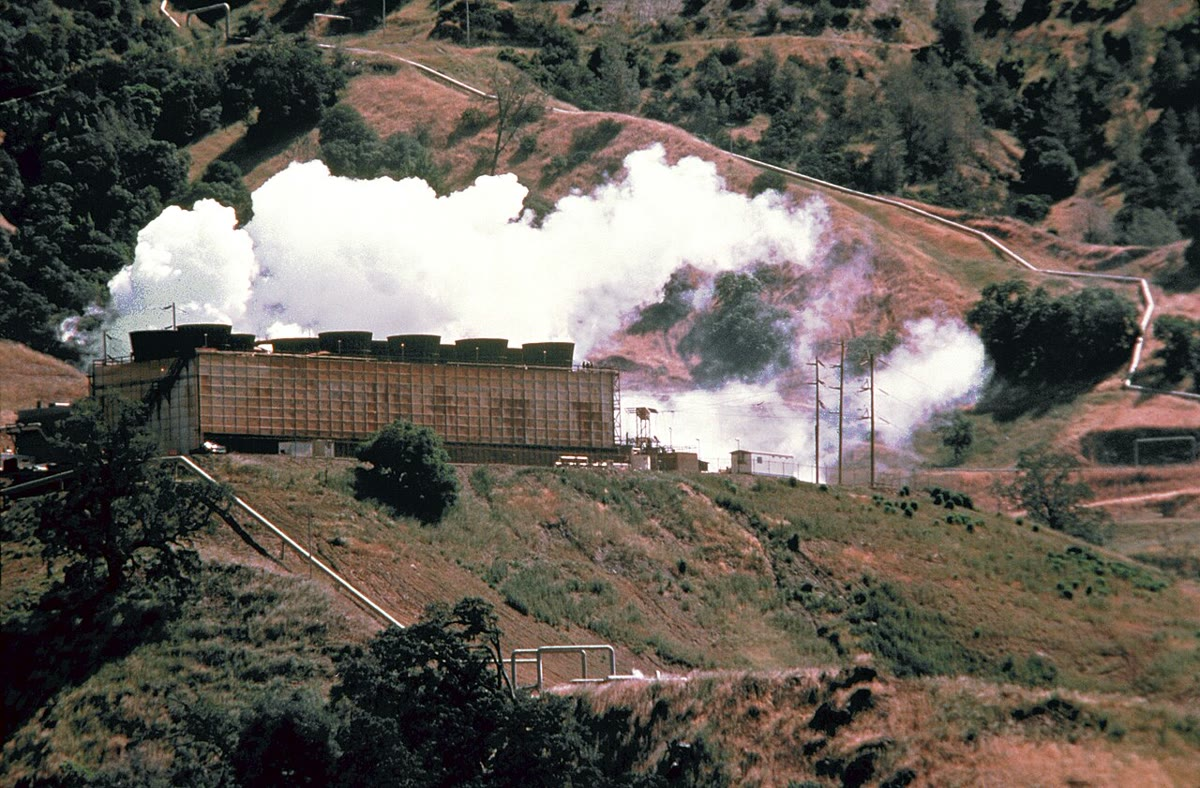
\includegraphics[width=\linewidth]{images/book4/b2-30-geyserville.jpg}
\end{minipage}
\par\smallskip{\small Izquierda: un \omterm{def:b2:energy-geology:geothermal}{sistema geotérmico} de alta entalpía (esquema, sin escala): el agua
recargada en los márgenes (azul) se calienta sobre una intrusión y asciende por un yacimiento fracturado
(rojo) hasta una fuente termal; los pozos captan el yacimiento. Derecha: una central geotérmica cerca de Geyserville,
California, en 1982, con tuberías de vapor en la ladera. Fotografía: U.S. Department of Defense
(dominio público).}
\end{omfigure}
% ledger: photo:b2-30-geyserville, usgs08g:egs

\begin{definition}[Sismicidad inducida]\label{def:b2:energy-geology:induced}
La \emph{sismicidad inducida}\index{sismicidad inducida} es la actividad sísmica causada por operaciones
humanas que modifican el esfuerzo o la presión del fluido intersticial en la corteza, con mayor frecuencia la
inyección de fluido en el subsuelo.
\end{definition}

El mecanismo es el criterio de Coulomb con presión de fluido intersticial: una falla desliza cuando el esfuerzo de cizalla
alcanza $\mu(\sigma_n - p)$, de modo que aumentar $p$ acerca a la rotura una falla que ya está cargada
sin ningún cambio de la carga tectónica. En los años sesenta, los fluidos residuales inyectados en el basamento
precámbrico fracturado bajo el Rocky Mountain Arsenal, cerca de Denver, a profundidades de 3.7 a
\qty{7.0}{km}, desencadenaron terremotos; quedaron confinados a la parte del yacimiento donde la
presión había aumentado más de \qty{32}{bar} (\qty{3.2}{MPa}). El fuerte aumento de los terremotos
de Oklahoma se ha atribuido a la eliminación de aguas residuales: cuatro pozos de gran
volumen podrían explicar una quinta parte de la sismicidad del centro de los Estados Unidos y desencadenar
terremotos a más de \qty{30}{km} de distancia. La estimulación de un yacimiento EGS eleva la presión intersticial del
mismo modo, de forma deliberada.
% ledger: hb81:denver, keranen:oklahoma, usgs08g:egs

\section{Uranio}\label{sec:b2:energy-geology:uranium}

Dos \omterm{def:b2:ore-deposits:types}{tipos de yacimiento} ilustran cómo se concentra el uranio: uno en una antigua discordancia y el
otro en areniscas.

\begin{definition}[Yacimientos de uranio de discordancia y de frente de oxidación]\label{def:b2:energy-geology:uranium}
Un \emph{yacimiento de uranio de discordancia}\index{yacimiento de uranio de discordancia} es un cuerpo
de pechblenda y uraninita que rellena fracturas y brechas en pelitas carbonosas metamorfizadas y
en las cuarzoarenitas suprayacentes, por debajo, por encima o a través de una discordancia entre rocas del \omterm{def:b2:precambrian-earth:eons}{Proterozoico}
inferior y medio en una \omterm{def:b2:basins-compared:types}{cuenca intracratónica}. Un \emph{yacimiento de uranio de frente de oxidación}\index{yacimiento de uranio de frente de oxidacion@yacimiento de uranio de frente de oxidación}
(roll front) es un cuerpo de minerales de uranio en forma de media luna que corta la estratificación de una
arenisca feldespática o tobácea en el límite entre terreno oxidado y terreno reducido, donde el
uranio se depositó en un ambiente localmente reductor, entre pirita.
\end{definition}

Los yacimientos de discordancia están alojados en rocas de 1800 a \qty{1200}{\Ma}, las pelitas metamorfizadas
por debajo de la discordancia y las areniscas no metamorfizadas por encima; sus rocas encajantes están cloritizadas, y los esquistos grafitosos que
acompañan a muchos de ellos son buenos conductores eléctricos, un objetivo de las prospecciones electromagnéticas. Key
Lake, Cluff Lake y Rabbit Lake, en Saskatchewan, y Jabiluka y Ranger, en el norte de Australia, son
ejemplos. Los frentes de oxidación son más recientes, sobre todo terciarios: en areniscas alimentadas por ceniza volcánica félsica o por
granito, los minerales de hierro oxidados quedan buzamiento arriba del frente y los reducidos buzamiento abajo, como en las cuencas
de Wyoming y de la costa del golfo de Texas.
% ledger: b1693:unconformity, b1693:sandstone

\begin{proposition}[El uranio 235 en el pasado]\label{prop:b2:energy-geology:u235}
Sean $r_0$ la razón atómica actual $^{235}$U/$^{238}$U y $\lambda_5$, $\lambda_8$ las constantes de
desintegración de los dos isótopos. Hace un tiempo $t$, la razón era
\begin{equation}
r(t) = r_0\,e^{(\lambda_5 - \lambda_8)\,t} ,
\label{eq:b2:energy-geology:u235}
\end{equation}
y el $^{235}$U constituía una fracción $r/(1 + r)$ de los átomos de uranio, despreciando la traza de
$^{234}$U.
\end{proposition}

\begin{proof}
Cada isótopo se desintegra exponencialmente: $N_5(\text{hoy}) = N_5(t)\,e^{-\lambda_5 t}$ y $N_8(\text{hoy})
= N_8(t)\,e^{-\lambda_8 t}$. Dividiendo, $r_0 = r(t)\,e^{-(\lambda_5 - \lambda_8)t}$.
\end{proof}

Con $\lambda_5 = \qty{9.8485e-10}{yr^{-1}}$, $\lambda_8 = \qty{1.55125e-10}{yr^{-1}}$ y las
abundancias actuales \qty{0.7204}{\percent} y \qty{99.2742}{\percent}, $r_0 = 0.0072567$; hace \qty{2.0}{\Ga}
$r = 0.0381$ y el uranio natural contenía un \qty{3.67}{\percent} de $^{235}$U, cinco veces la proporción
actual.
% ledger: amherst:constants, iaea:isotopes
% values: r 0.038144, 3.6743 % (calc/ch30.py)

\begin{history}[Un reactor de dos mil millones de años]
En 1972, científicos franceses que medían mineral de uranio encontraron déficits pequeños pero significativos de
$^{235}$U, que rastrearon hasta la mina de Oklo, en Gabón. Allí, bolsadas de roca contenían hasta un
\qty{65}{\percent} de uranio con apenas la mitad de la proporción normal de $^{235}$U, y neodimio
empobrecido en su isótopo primordial $^{142}$Nd pero enriquecido en los isótopos 143 a 150 que produce la fisión:
en la mena se habían producido reacciones en cadena hace unos dos mil millones de años, a unos \qty{300}{bar}
y de 400 a \qty{500}{\celsius}. Se conocen dieciséis de estos reactores naturales en Oklo y en la cercana
Bangombé, los dos únicos yacimientos del mundo donde se han encontrado; la materia orgánica había contribuido a
concentrar el uranio, y el óxido de uranio ha retenido en su lugar desde entonces la mayor parte de los actínidos y de los
productos de fisión no volátiles.
\end{history}
% ledger: oklo:curtis, oklo:cowan, oklo:gl96, oklo:nagy

\section{Almacenamiento geológico de dióxido de carbono}\label{sec:b2:energy-geology:ccs}

\begin{definition}[Almacenamiento geológico de \ce{CO2}, mecanismos de retención, factor de eficiencia de almacenamiento]\label{def:b2:energy-geology:ccs}
El \emph{almacenamiento geológico de \ce{CO2}}\index{almacenamiento geológico de CO$_2$} es la inyección de dióxido
de carbono en formaciones rocosas porosas a gran profundidad, yacimientos agotados de petróleo y gas, formaciones salinas
profundas o capas de carbón, para su retención durante largos periodos. Los \emph{mecanismos de retención
del \ce{CO2}}\index{mecanismos de retención del CO$_2$} que lo inmovilizan son la retención estructural (y estratigráfica)
bajo una roca sello; la retención residual, como fase inmóvil retenida en los poros por fuerzas
capilares; la retención por solubilidad, por disolución en el agua de formación; la retención mineral, por reacción
con minerales que forma carbonatos; y, en el carbón y las lutitas, la adsorción sobre la materia orgánica. El \emph{factor de eficiencia de almacenamiento}\index{factor de eficiencia de almacenamiento}
$E$ de una formación es la fracción de su volumen de poros que cabe esperar que llene el
\ce{CO2} inyectado.
\end{definition}
% ledger: srccs:retention, netl08:saline

El dióxido de carbono es un gas en superficie, pero su punto crítico está a \qty{31.0}{\celsius} y
\qty{7.38}{MPa}. A lo largo de una geoterma de \qty{25}{\celsius\per\km} desde \qty{15}{\celsius} con
presión hidrostática, la temperatura supera el valor crítico a \qty{641}{m} y la presión a
\qty{742}{m}; la densidad del \ce{CO2} puro pasa bruscamente de \qty{234}{kg.m^{-3}} (a \qty{700}{m}) a
\qty{583}{kg.m^{-3}} (a \qty{900}{m}), y después se estabiliza entre 670 y \qty{700}{kg.m^{-3}} por debajo de
\qty{1.5}{km}. Una tonelada ocupa \qty{534}{m^3} en superficie y \qty{1.6}{m^3} a \qty{1000}{m},
330 veces menos; por eso las evaluaciones de almacenamiento solo consideran formaciones a más de
\qty{800}{m} de profundidad.
% ledger: nist:co2-critical, data:b4-co2-density, srccs:density, netl08:saline
% values: z_tc 641.2 m, z_pc 742.2 m; volume ratio 331.9 (figdata co2_density.py numbers)

\begin{omfigure}
\centering
\begin{minipage}[b]{0.49\linewidth}\centering
\begin{tikzpicture}
\begin{axis}[omrecord, width=0.95\linewidth, height=5.2cm, xmin=0, xmax=750, ymin=0, ymax=3,
  y dir=reverse, xlabel={densidad del \ce{CO2} (\unit{kg.m^{-3}})}, ylabel={profundidad (km)},
  tick label style={font=\scriptsize}, label style={font=\small}]
% computed in figdata/bachelor-2/co2_density.py part profile; ledger: data:b4-co2-density
\addplot[black!45, densely dashed] coordinates {(0,0.742) (750,0.742)};
\node[font=\tiny, text=black!60, anchor=south east] at (axis cs:745,0.73) {presión crítica};
\addplot[omDef, line width=1.1pt, mark=*, mark size=0.9pt] table[x=rho, y expr=\thisrow{depth_m}/1000] {figdata/out/bachelor-2-co2_density-profile.dat};
\end{axis}
\end{tikzpicture}
\end{minipage}\hfill
\begin{minipage}[b]{0.49\linewidth}\centering
\begin{tikzpicture}
\begin{axis}[width=0.95\linewidth, height=5.2cm, xmin=0, xmax=4, ymin=0, ymax=100,
  axis x line=bottom, axis y line=left, axis line style={-}, axis on top,
  xlabel={tiempo tras la inyección (años)}, ylabel={parte del \ce{CO2} almacenado},
  xtick={0,1,2,3,4}, xticklabels={1,10,100,1000,$10^4$}, ytick=\empty,
  tick label style={font=\scriptsize}, label style={font=\small}]
% schematic, after IPCC SRCCS (2005) Figure 5.9; ledger: srccs:trapping
% bands from the bottom: mineral, solubility, residual, structural (cumulative tops 0/0/1/5/15,
% 2/8/21/40/60, 10/30/56/80/90, 100)
\fill[omLithLime!60!black] (axis cs:0,0) -- (axis cs:1,0) -- (axis cs:2,1) -- (axis cs:3,5) -- (axis cs:4,15) -- (axis cs:4,0) -- cycle;
\fill[omDef!40] (axis cs:0,0) -- (axis cs:1,0) -- (axis cs:2,1) -- (axis cs:3,5) -- (axis cs:4,15) -- (axis cs:4,60) -- (axis cs:3,40) -- (axis cs:2,21) -- (axis cs:1,8) -- (axis cs:0,2) -- cycle;
\fill[omProp!40] (axis cs:0,2) -- (axis cs:1,8) -- (axis cs:2,21) -- (axis cs:3,40) -- (axis cs:4,60) -- (axis cs:4,90) -- (axis cs:3,80) -- (axis cs:2,56) -- (axis cs:1,30) -- (axis cs:0,10) -- cycle;
\fill[black!15] (axis cs:0,10) -- (axis cs:1,30) -- (axis cs:2,56) -- (axis cs:3,80) -- (axis cs:4,90) -- (axis cs:4,100) -- (axis cs:0,100) -- cycle;
\node[font=\scriptsize] at (axis cs:1.1,72) {estructural};
\node[font=\scriptsize] at (axis cs:2.1,38) {residual};
\node[font=\scriptsize] at (axis cs:3.1,22) {solubilidad};
\node[font=\scriptsize, text=white, anchor=south east] at (axis cs:3.98,0.5) {mineral};
\end{axis}
\end{tikzpicture}
\end{minipage}
\par\smallskip{\small Izquierda: densidad del \ce{CO2} puro en función de la profundidad a lo largo de una geoterma de
\qty{25}{\celsius\per\km} desde \qty{15}{\celsius}, con presión hidrostática. Datos: NIST Chemistry
WebBook (ecuación de estado de Span--Wagner), en las condiciones del Informe especial del IPCC sobre la captación y el
almacenamiento de dióxido de carbono (2005). Derecha: cómo se reparten los mecanismos de retención el \ce{CO2} almacenado
a lo largo del tiempo (esquema, según el mismo informe): la retención por la roca sello da paso a las formas residual,
disuelta y mineral, que son menos móviles.}
\end{omfigure}

\begin{proposition}[Capacidad de almacenamiento de una formación]\label{prop:b2:energy-geology:capacity}
Una formación de superficie $A$, espesor $h$ y porosidad $\phi$, en la que el \ce{CO2} tiene la densidad $\rho$
y el \omterm{def:b2:energy-geology:ccs}{factor de eficiencia de almacenamiento} es $E$, puede almacenar la masa
\begin{equation}
M = A\,h\,\phi\,\rho\,E .
\label{eq:b2:energy-geology:capacity}
\end{equation}
En un campo petrolífero agotado que ha producido un volumen en condiciones de tanque $N_p$, sustituir el petróleo producido
volumen por volumen da $M = \rho\,N_p\,B_o$.
\end{proposition}

\begin{proof}
El volumen de poros es $Ah\phi$, del que el \ce{CO2} llena una fracción $E$, con densidad $\rho$. En el
campo petrolífero, el petróleo producido ocupaba $N_pB_o$ en el yacimiento, el volumen que pasa a ocupar el \ce{CO2}.
\end{proof}

En las formaciones salinas profundas, las simulaciones dan $E$ entre el 1 y el \qty{4}{\percent} del volumen de poros
para un intervalo de confianza del 15 al 85 por ciento, con una mediana cercana al \qty{2}{\percent}: la mayor parte del espacio
poroso nunca se alcanza o conserva su agua. Una formación de \qty{1000}{km^2}, de \qty{50}{m} de espesor y de
porosidad 0.20 a \qty{2000}{m} ($\rho = \qty{686}{kg.m^{-3}}$) almacena \qty{137}{Mt} con $E =
\qty{2}{\percent}$.
% ledger: netl08:saline, data:b4-co2-density
% values: 1e9*50*0.2*686*0.02 = 1.372e11 kg (calc/ch30.py)

Una vez inyectado, el \ce{CO2} asciende bajo la roca sello y se extiende. Detrás de la pluma que migra, las fuerzas
capilares retienen saturaciones residuales que pueden alcanzar del 15 al \qty{25}{\percent} del espacio poroso;
la disolución absorbe de 20 a \qty{60}{kg} de \ce{CO2} por metro cúbico de agua de formación y, en
formaciones de flujo lento, hasta el \qty{30}{\percent} del \ce{CO2} inyectado se disuelve en unas decenas de
años. La retención por solubilidad domina durante decenas a cientos de años, las formas iónicas durante cientos a
miles, la retención mineral durante miles a millones: las reacciones con minerales carbonatados duran días,
con silicatos, de cientos a miles de años. El almacenamiento se vuelve más seguro con el tiempo, y en
emplazamientos bien elegidos y bien gestionados se juzgó probable la retención del \qty{99}{\percent} o más del \ce{CO2} durante
1000 años.
% ledger: srccs:trapping, srccs:retention

\begin{dated}{2005}
En Sleipner, en el mar del Norte, a unos \qty{250}{km} de la costa de Noruega, el \ce{CO2} separado del
gas natural del campo, alrededor del \qty{9}{\percent} de este, se inyecta desde octubre de 1996 en
la formación Utsira, una arenisca salina no consolidada situada de 800 a \qty{1000}{m} por debajo del fondo marino,
a razón de alrededor de \qty{1}{Mt} al año. A comienzos de 2005 se habían almacenado más de \qty{7}{Mt}, de las \qty{20}{Mt}
previstas durante la vida del proyecto. Campañas sísmicas repetidas obtienen imágenes de la pluma, cuya huella era entonces
de unos \qty{5}{km^2}, y muestran que la roca de cobertera que la cubre la sella.
\end{dated}
% ledger: srccs:sleipner

\begin{inthefield}[Leer un pozo mientras se perfora]
\centering
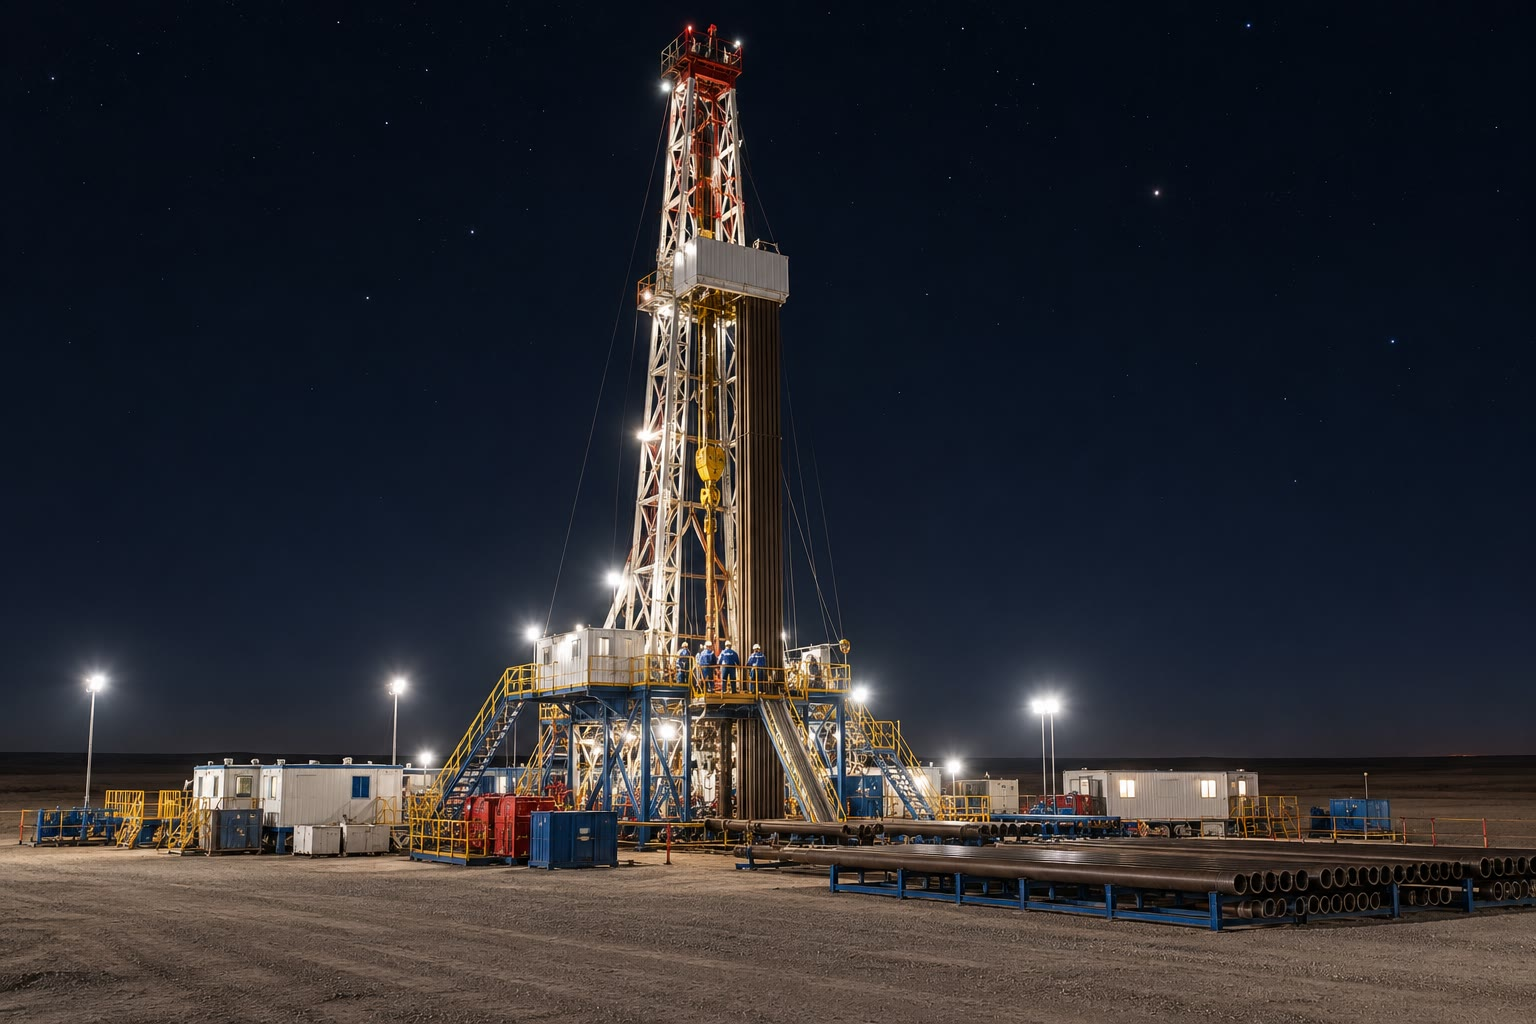
\includegraphics[width=0.56\linewidth]{images/book4/ai/b2-rig-night.jpg}
\par\smallskip{\small Una torre de perforación terrestre de noche (ilustración generada por IA).}
\par\medskip\raggedright
Cuando se termina un tramo de un pozo, los geofísicos bajan herramientas con un cable y registran en función de la
profundidad las propiedades de las rocas que rodean el sondeo. Una registra su radiactividad natural, baja en
la arenisca y más alta en la lutita; otra, su densidad aparente, de la que se deduce la porosidad como
(densidad de grano $-$ densidad aparente)/(densidad de grano $-$ densidad del fluido), con \qty{2.65}{g/cm^3} para
los granos de cuarzo y alrededor de \qty{1}{g/cm^3} para el agua. Leídos juntos, estos registros de sondeo dan el
espesor neto de la roca almacén y la porosidad que entran en las fórmulas volumétricas de este capítulo.
\end{inthefield}
% ledger: keys:gamma, keys:density-porosity

\section*{Ejercicios}\label{sec:b2:energy-geology:exercises}

Datos de los ejercicios, salvo aviso contrario: $R = \qty{8.314}{J.mol^{-1}.K^{-1}}$; un millón de
años son \qty{3.156e13}{s}; querógeno de Green River, $A = \qty{9.21e13}{s^{-1}}$, $E/R = \qty{26800}{K}$;
masas atómicas C 12.011, H 1.008, O 15.999; densidad del \ce{CO2} a lo largo del perfil de la figura:
\qty{1.872}{kg.m^{-3}} en superficie, 583 a \qty{900}{m}, 621 a \qty{1000}{m}, 686 a
\qty{2000}{m}. Redondéese a tres cifras significativas.
% ledger: codata:R, fp14:gr-daem, data:b4-co2-density

\begin{exercise}[$\star$]\label{exo:b2:energy-geology:1}
(a) Cuatro querógenos inmaduros tienen razones atómicas H/C de 1.58, 0.95, 1.24 y 1.12. Asígnese a cada uno un tipo y dígase
cuál produciría sobre todo gas. (b) Compruébense las razones H/C y O/C de la fórmula
C$_{100}$H$_{150}$N$_3$O$_8$S. (c) Hállense a partir de la composición en masa C \qty{77.4}{\percent}, H
\qty{9.8}{\percent}, O \qty{8.2}{\percent}.
\end{exercise}

\begin{exercise}[$\star$]\label{exo:b2:energy-geology:2}
(a) Cinco muestras de una roca generadora de tipo~II tienen $R_o$ = 0.45, 0.68, 1.1, 1.6 y \qty{2.5}{\percent}.
Descríbase el estado de cada una respecto del petróleo y del gas. (b) ¿Genera metano un querógeno de tipo~III con $R_o =
\qty{0.68}{\percent}$? (c) ¿Qué fracción convertida $F$ de Easy\%Ro corresponde a
$R_o = 0.6$ y al \qty{1.3}{\percent}?
\end{exercise}

\begin{exercise}[$\star$]\label{exo:b2:energy-geology:3}
Una trampa cubre \qty{6}{km^2}; su roca almacén tiene \qty{25}{m} de espesor neto, porosidad 0.18 y saturación de agua
0.30, y $B_o = 1.25$. (a) Hállense el volumen de petróleo en el yacimiento y el STOIIP. (b) Hállese
el volumen producido para \omterm{def:b2:energy-geology:volumetrics}{factores de recuperación} de 0.30 y 0.40.
\end{exercise}

\begin{exercise}[$\star$]\label{exo:b2:energy-geology:4}
Un acuífero de arenisca de \qty{200}{m} de espesor bajo \qty{10}{km^2} está a \qty{75}{\celsius}. (a) Hállese su
\omterm{def:b2:energy-geology:geothermal}{calor in situ} por encima de \qty{15}{\celsius}, con $C = \qty{2.5}{MJ.m^{-3}.K^{-1}}$. (b) ¿A qué
clase de entalpía pertenece? (c) Hállese la potencia térmica media durante 30 años para $R_g = 0.25$.
\end{exercise}

\begin{exercise}[$\star\star$]\label{exo:b2:energy-geology:5}
(a) Hállese la energía de activación para la que una velocidad de Arrhenius se duplica entre 100 y
\qty{110}{\celsius}. (b) ¿En qué factor aumenta la velocidad de la reacción de Green River en el mismo
intervalo? (c) ¿Cuál de las dos reglas da más peso al tiempo que una roca pasó a baja temperatura,
y qué implica esto para un TTI calculado para una roca generadora de tipo~I?
\end{exercise}

\begin{exercise}[$\star\star$]\label{exo:b2:energy-geology:6}
(a) Demuéstrese a partir de \eqref{eq:b2:energy-geology:maturation} que la temperatura de semitransformación cumple
$T = (E/R)\big/\ln\bigl[A T^2/(\beta\,(E/R)\ln 2)\bigr]$, y resuélvase por iteración para el querógeno de Green
River calentado a \qty{1}{\celsius\per\Myr} y a \qty{10}{K} por minuto. (b) Compárese la
diferencia con la estimación $(RT^2/E)\ln(\beta_2/\beta_1)$ tomada a la temperatura más baja, y
explíquese la discrepancia.
\end{exercise}

\begin{exercise}[$\star\star$]\label{exo:b2:energy-geology:7}
Con \eqref{eq:b2:energy-geology:u235} y los datos del texto: (a) hállese la proporción de $^{235}$U en el
uranio natural hace \qty{2.0}{\Ga} y hace \qty{1.8}{\Ga}; (b) ¿cuándo era del \qty{3.00}{\percent}?
(c) La mena de Oklo contiene tan solo la mitad de la proporción normal actual de $^{235}$U. Sin tener en cuenta el $^{238}$U
consumido, ¿qué fracción del $^{235}$U presente en el momento de las reacciones se fisionó, y
por qué la desintegración posterior no cambia la respuesta?
\end{exercise}

\begin{exercise}[$\star\star$]\label{exo:b2:energy-geology:8}
(a) Hállese el volumen de \qty{1}{Mt} de \ce{CO2} en superficie, a \qty{1000}{m} y a
\qty{2000}{m}. (b) En Sleipner se habían inyectado más de \qty{7}{Mt} en 2005, a unos
\qty{900}{m}, en una pluma de \qty{5}{km^2} de huella. Tomando una porosidad de 0.35 y una saturación de \ce{CO2}
de 0.30 en la pluma, hállense el volumen de roca que ocupa y su espesor medio.
\end{exercise}

\begin{exercise}[$\star\star$]\label{exo:b2:energy-geology:9}
Un yacimiento de alta entalpía mide $3 \times 2 \times \qty{1.5}{km}$ y está a \qty{250}{\celsius}, con
$C = \qty{2.6}{MJ.m^{-3}.K^{-1}}$. (a) Hállese su \omterm{def:b2:energy-geology:geothermal}{calor in situ} por encima de \qty{15}{\celsius}. (b) Hállese la
potencia térmica media durante 30 años para $R_g = 0.1$ y $0.25$. (c) Su campo cubre \qty{6}{km^2};
a razón de 10 a \qty{20}{MW} de electricidad por kilómetro cuadrado, ¿qué fracción de la potencia térmica con
$R_g = 0.1$ se convierte en electricidad?
\end{exercise}

\begin{exercise}[$\star\star\star$]\label{exo:b2:energy-geology:10}
Una falla a unos \qty{4}{km} soporta un esfuerzo normal de \qty{80}{MPa} y un esfuerzo de cizalla de
\qty{22}{MPa}; su coeficiente de rozamiento es 0.6 y la presión intersticial es hidrostática,
\qty{39}{MPa}. (a) ¿Es estable la falla? Hállese el aumento de presión intersticial que la lleva a la rotura, en
megapascales y en bares, y compárese con el umbral de Denver. (b) Lo mismo si el esfuerzo de cizalla es de
\qty{24}{MPa}. (c) Explíquese por qué pueden desencadenarse terremotos a kilómetros de un pozo de inyección,
y años después de que empezara la inyección.
\end{exercise}

\begin{exercise}[$\star\star\star$]\label{exo:b2:energy-geology:11}
(a) A partir de la aproximación de \eqref{eq:b2:energy-geology:maturation}, demuéstrese que, con una velocidad de
calentamiento constante, la tasa de transformación pasa del \qty{10}{\percent} al \qty{90}{\percent} en un
intervalo de temperatura $\Delta T \approx \bigl[\ln\ln 10 - \ln\ln(10/9)\bigr]\,RT^2/E$. (b) Evalúese
para el querógeno de Green River a \qty{1}{\celsius\per\Myr}. (c) Compárese con la curva continua de la
figura y explíquese la diferencia.
\end{exercise}

\begin{exercise}[$\star\star\star$]\label{exo:b2:energy-geology:12}
Sleipner debe almacenar \qty{20}{Mt} de \ce{CO2}. (a) Hállese el volumen de agua de formación necesario para
disolverlo todo, a 20 y a \qty{60}{kg.m^{-3}}. (b) Hállese su volumen como fase libre a
\qty{1000}{m}. (c) Con $E = \qty{2}{\percent}$, hállense el volumen de poros de formación necesario y
la superficie de una formación de \qty{50}{m} de espesor y porosidad 0.30.
\end{exercise}
% ledger: srccs:trapping, srccs:sleipner, hb81:denver

\begin{problem}[{Problema de fin de semana --- Una cuenca, dos usos}]\label{pb:b2:energy-geology:1}
En una cuenca inventada, una roca generadora de tipo~I se depositó hace \qty{120}{\Ma} en la superficie.
Después se acumuló sedimento a \qty{60}{m} por millón de años hasta hace \qty{70}{\Ma}, y a \qty{30}{m}
por millón de años desde entonces. La superficie está a \qty{15}{\celsius} y la geoterma es constante, de
\qty{25}{\celsius\per\km}. El querógeno tiene la cinética de Green River del texto (energía única).
Su cocina, la parte madura de la roca generadora, cubre \qty{400}{km^2}, tiene \qty{50}{m} de espesor y
una densidad de \qty{2400}{kg.m^{-3}}, y puede producir \qty{30}{kg} de petróleo por tonelada de roca con transformación
completa; el petróleo tiene una densidad en superficie de \qty{850}{kg.m^{-3}}. El petróleo llena una trampa de
\qty{12}{km^2} cuya roca almacén, centrada a \qty{2000}{m}, tiene un espesor neto de \qty{40}{m},
porosidad 0.22 y saturación de agua 0.25, con $B_o = 1.30$. Úsense los datos de los ejercicios; redondéese a
tres cifras significativas.

\noindent\textbf{Parte I --- Enterramiento e índice tiempo--temperatura.}
\begin{enumerate}
  \item Hállense la profundidad y la temperatura de la roca generadora hace \qty{70}{\Ma} y hoy.
  \item Hállese su velocidad de calentamiento en cada fase.
  \item Hállese el tiempo que pasó en cada intervalo de \qty{10}{\celsius}, desde \qty{15}{\celsius} hasta
        su temperatura actual.
  \item Calcúlese su TTI actual (método del texto).
  \item ¿Cuándo, a qué temperatura y a qué profundidad superó un TTI de 15?
  \item Lo mismo para 75 y 160.
  \item Según el TTI, ¿sigue generando petróleo la roca generadora?
\end{enumerate}

\noindent\textbf{Parte II --- Transformación según la cinética.}
\begin{enumerate}[resume]
  \item Hállese la constante de velocidad a \qty{90}{\celsius} y demuéstrese que menos del \qty{0.2}{\percent} del
        querógeno pudo transformarse antes de hace \qty{70}{\Ma}.
  \item Con \eqref{eq:b2:energy-geology:maturation} y la velocidad de calentamiento de la segunda fase,
        hállense la fracción sin transformar y la tasa de transformación actuales.
  \item Hállese la temperatura de semitransformación con esta velocidad de calentamiento (\cref{exo:b2:energy-geology:6}).
  \item ¿Cuándo se alcanzó?
  \item Compárese con el momento del máximo de generación que da el TTI, y explíquese la diferencia.
  \item ¿Un querógeno de tipo~II con una energía de activación media más baja se habría transformado antes o después?
\end{enumerate}

\noindent\textbf{Parte III --- Petróleo generado, in situ y recuperable.}
\begin{enumerate}[resume]
  \item Tomando una tasa de transformación de 0.92, hállese la masa de petróleo generada en la cocina.
  \item Hállese su volumen en superficie.
  \item Hállese el STOIIP de la trampa.
  \item ¿Qué fracción del petróleo generado contiene la trampa? Consérvense \qty{1.56e9}{m^3} para (15).
  \item Hállese el petróleo producido para un \omterm{def:b2:energy-geology:volumetrics}{factor de recuperación} de 0.35.
  \item ¿Por qué el \omterm{def:b2:energy-geology:volumetrics}{factor de recuperación} es mucho menor que uno, y qué cambiaría la inyección de \ce{CO2}?
\end{enumerate}

\noindent\textbf{Parte IV --- El campo agotado como almacén de \ce{CO2}.}
\begin{enumerate}[resume]
  \item Hállense la temperatura y la presión hidrostática de la roca almacén. ¿Es supercrítico allí el \ce{CO2}
        inyectado? Léase su densidad en la figura.
  \item Conservando $N_p = \qty{2.13e7}{m^3}$, hállese el volumen de yacimiento liberado por la producción.
  \item Exprésese como \omterm{def:b2:energy-geology:ccs}{factor de eficiencia de almacenamiento} del volumen de poros de la trampa, y compárese con
        las formaciones salinas.
  \item Una formación salina bajo el campo cubre \qty{600}{km^2}, tiene \qty{80}{m} de espesor y
        porosidad 0.20, con \ce{CO2} a \qty{691}{kg.m^{-3}}. Hállese su capacidad con $E =
        \qty{2}{\percent}$.
  \item ¿Cuántos años de inyección al ritmo de Sleipner la llenarían?
  \item Con $\rho = \qty{686}{kg.m^{-3}}$ y el volumen liberado redondeado a \qty{2.77e7}{m^3}, hállese
        la capacidad de almacenamiento de \ce{CO2} del yacimiento agotado, en megatoneladas.
\end{enumerate}
\end{problem}
% ledger: fp14:gr-daem, waples80:tti, hamm14:tti-table, netl08:oilgas, netl08:saline, data:b4-co2-density, nist:co2-critical, srccs:sleipner
